\subsection{实验对象与数据划分}
第\ref{sec:fixed_method}节导出的式（36）引出两个递进问题：格式本身在变质量与阻尼下是否具备预期的收敛阶与几何结构特性，以及在其保守轨迹上实复参数化与二次物理先验如何影响长期预测。实验据此在光滑标量振子与两模态磁驱梁两个层次上展开。

对$N$个广义坐标，$q,p\in\mathbb R^N$，质量矩阵$M(q)\in\mathbb R^{N\times N}$，状态$z=(q,p)\in\mathbb R^{2N}$；$K,C,\epsilon$与$M$同阶，$\Delta,F_{\rm ext}$为$N$维向量。因此$N=1$对应标量质量和二维相空间，$N=2$对应$2\times2$质量矩阵和四维相空间。各矩阵积保持式（36）的次序，分母按左侧线性求解处理。

标量诊断设常质量（$m=k=1$）与变质量（$M(q)=1+0.3q^2$、$K(q)=1+0.4q^2$）两组无量纲算例，每组分别取$C=0$与$C=0.2$（$F_{\mathrm{ext}}=0$）以分离质量变化与阻尼效应；变质量项按式（35）中点约定隐式迭代至固定容差，参照解分别由矩阵指数与高精度DOP853取得。学习实验则采用固支自由、小斜率两模态磁驱梁：杆长$80\,\mathrm{mm}$、半径$0.6\,\mathrm{mm}$、Young模量$5\,\mathrm{MPa}$、密度$1100\,\mathrm{kg/m^3}$、磁偶极矩$2\times10^{-5}\,\mathrm{A\,m^2}$、静态偏置磁场$0.03\,\mathrm T$。实验取常质量保守分支（接触、阻尼与时变输入置零），正则状态为$x=(X_1,X_2,Y_1,Y_2)$，无量纲时间$\tau=\omega_0t$（$\omega_0=11.4172873\,\mathrm{rad/s}$），目标能量为
\begin{equation}
 \begin{aligned}
 h_*(x)={}&\frac12\sum_{j=1}^{2}\nu_j(X_j^2+Y_j^2)\\
          &+1-\cos(d^TX)-\frac12(d^TX)^2,
 \end{aligned}
 \label{eq:learning-model}
\end{equation}
其中$\nu=(1,6.1521175)$、$d=(0.2256708,0.3217988)$，该正则尺度下动能系数$M^{-1}=\operatorname{diag}(\nu)$，完整保留末端偏角余弦磁势。固定五个独立随机种子（$17,43,91,137,211$），每个种子由互不重合初值生成12条训练（$2\,\mathrm s$）、4条验证（$4\,\mathrm s$）与8条测试轨迹（$40\,\mathrm s$），由式（36）以步长$h\approx0.01$生成并对齐物理终点；监督标签取一步差商配对\emph{该步中点状态}，并加入幅值不超过$10^{-6}$的独立均匀噪声。

\subsection{匹配解析特征与端到端网络}
实复比较分层推进以隔离坐标形式与网络优化。第一层匹配同一解析函数空间：无先验R、C同时拟合二次与高阶读出（45个自由实参数），有先验GR、GC固定已知二次能量而仅拟合非线性余项（35个自由实参数），采用相同正则化经线性最小二乘求解。

第二层训练全部隐藏层权重：实网络取$4$--$20$--$26$--$1$结构；复网络设两个16复通道隐藏层，采用复权重与实虚分通道$\tanh$激活\citep{Trabelsi2018}并以实值线性读出保守能量（$\mathcal H=H+i0$），二者严格对齐为673个实标量参数。四组端到端网络共享训练集RMS尺度、512批次大小与10000次Adam更新（初学习率$0.002$，在预算$1/2$与$3/4$处各乘$0.3$，每100步按独立验证集选最优权重），预测统一对实正则坐标求自动微分梯度并由同容差隐式中点积分推进。另设零可训参数纯二次物理基线$H_0=\tfrac12\sum_j\nu_j(X_j^2+Y_j^2)$，以精确Cayley中点变换推进同一测试集，用作品质参照而不改动原有五项配对。

\subsection{评价量与五项配对比较}
每条测试轨迹同步评估完整状态误差、杆端位移时间域RMSE（毫米）、相位偏差与能量变化，并分别对照式（36）同一步长离散教师与独立DOP853连续参考（端到端先逐轨迹求RMSE再跨8条轨迹平均，解析特征按全域均方根汇总）。为在不引入重训练变量的条件下剥离时间离散误差，进一步固定全部20组已选端到端权重，在$h,h/2,h/4,h/8$四档步长下重新推进同一批测试轨迹（覆盖$15.993\,\mathrm s$内914个对齐输出时刻），同步计算同一步长非线性教师与连续参考。

对任一误差指标$E$，在每个种子内构造五项配对差：
\begin{align}
 &E_R-E_{GR},\quad E_C-E_{GC},\nonumber\\
 &E_R-E_C,\quad E_{GR}-E_{GC},\nonumber\\
 &(E_{GR}-E_{GC})-(E_R-E_C),
 \label{eq:five-contrasts}
\end{align}
前两项度量物理先验收益，中间两项度量同先验设置下的实复差异，末项度量二者交互；表格汇总五种子的均值与样本标准差。

\subsection{差分格式的收敛与结构诊断}
标量诊断（表\ref{tab:convergence}、图\ref{fig:diagnostics}）确认四类光滑算例在最细两档步长下均呈近二阶收敛（变质量参考容差加密波动在$10^{-13}$量级）；常质量保守振子二次能量漂移约$3.44\times10^{-14}$，阻尼振子离散功率平衡残差约$1.84\times10^{-16}$。

但阻尼工况的几何结构表现迥异：在$m=k=1$、$c=0.2$、$h=0.1$下，式（36）一步映射行列式为$0.980246913580247$，偏离连续时变Birkhoff二形式对应的$\exp(-ch)=0.980198673306755$，归一化结构缺陷达$4.92\times10^{-5}$（精确流仅约$1.11\times10^{-16}$），印证了线性阻尼中点格式不保持相应时变Birkhoff二形式的结论\citep[第15章，第630页，式(5.4)]{FengQin2010}，也支持后续采用常质量保守分支生成学习数据。

为检验非单位质量与矩阵耦合，另设六类无量纲保守基准：$N=1$取常质量$m=1,2,5$及$m(q)=2+0.3q^2$；$N=2$取常矩阵$M_0$及$M(q)=M_0+0.3qq^T$，其中
\[
 M_0=\begin{pmatrix}2&0.3\\0.3&1.5\end{pmatrix},\qquad
 K_0=\begin{pmatrix}1.7&0.2\\0.2&0.9\end{pmatrix}.
\]
势能统一写为$V=\tfrac12q^TK_0q+\tfrac\beta4\|q\|^4$，标量时$K_0=1$，常质量组取$\beta=0$、变质量组取$\beta=0.1$。这些是格式检验用的数学算例；两模态梁的物理参数仍采用前述定义。对每类三个固定初值，以$h=0.2,0.1,0.05,0.025,0.0125$积分至$T=5$，参照解分别取矩阵指数和独立高精度连续积分。各组最细观察阶接近二阶（表\ref{tab:eq36_mass_dimension}）；全部90个首步切映射探针的最大辛缺陷为$4.58\times10^{-16}$。$M_0$与$K_0$不交换，错误右侧逆和逐元素倒数的单步偏差分别约为$4.54\times10^{-4}$与$0.105$，因此标量检验不能替代耦合矩阵核对。

\begin{table}[t]
\centering\small\setlength{\tabcolsep}{3pt}
\caption{式（36）的质量维度基准。$T=5$、最细步长$h=0.0125$；对每类三个固定初值报告最大终点误差、最小观察阶和最大首步探针辛缺陷。}
\label{tab:eq36_mass_dimension}
\begin{tabular}{lrrr}
\toprule
情形 & 状态误差 & 阶 & 辛缺陷\\
\midrule
$N=1,\ m=1$ & $4.74\times10^{-5}$ & $1.9999$ & $0$ \\
$N=1,\ m=2$ & $2.30\times10^{-5}$ & $2.0000$ & $1.11\times10^{-16}$ \\
$N=1,\ m=5$ & $5.88\times10^{-6}$ & $2.0000$ & $1.11\times10^{-16}$ \\
$N=1,\ m(q)$ & $2.40\times10^{-5}$ & $2.0000$ & $2.22\times10^{-16}$ \\
$N=2,\ M_0$ & $4.17\times10^{-5}$ & $1.9999$ & $1.13\times10^{-16}$ \\
$N=2,\ M(q)$ & $4.16\times10^{-5}$ & $1.9999$ & $2.24\times10^{-16}$ \\
\bottomrule
\end{tabular}
\end{table}


\begin{table*}[t]
\centering\small
\caption{固定时域$T=10$上的状态误差及观察阶。}
\label{tab:convergence}
\begin{tabular}{lrr}
\toprule
算例 & $h=0.025$的终点状态误差 & $h=0.05$至$0.025$的阶 \\
\midrule
常质量／保守 & $0.000520785$ & $1.999594$ \\
常质量／阻尼 & $0.000182687$ & $1.999938$ \\
变质量／保守 & $0.000463096$ & $1.999723$ \\
变质量／阻尼 & $0.00015273$ & $1.999983$ \\
\bottomrule
\end{tabular}

\end{table*}

\begin{figure*}[t]
\centering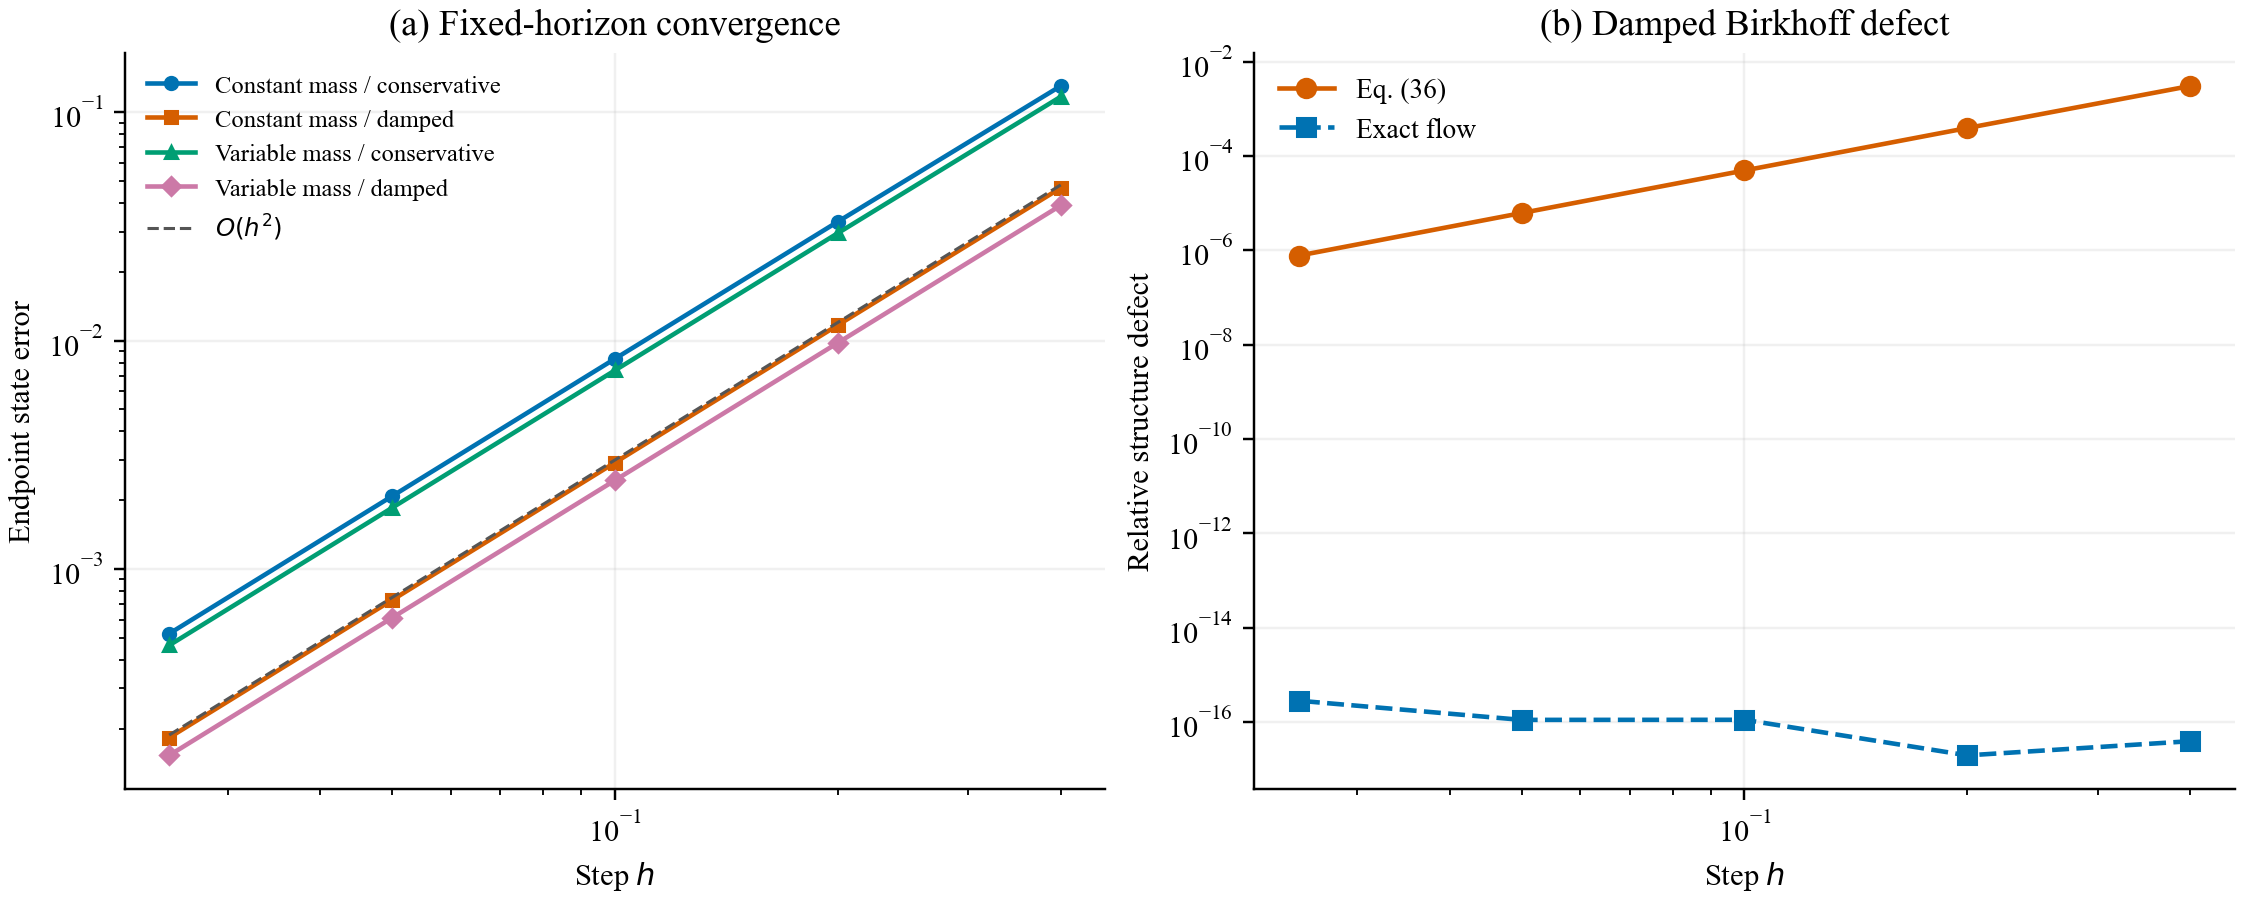
\includegraphics[width=0.96\textwidth]{equation36_diagnostics.png}
\caption{固定差分格式的标量诊断。左：固定时域$T=10$上的误差随步长变化。右：常质量阻尼算例的时变Birkhoff结构残差。该残差与精确流的对应值比较。}
\label{fig:diagnostics}
\end{figure*}

\subsection{学习结果与长期误差来源}
在第一层匹配解析特征的20次拟合与$40\,\mathrm s$预测中，相对离散教师，R/C杆端RMSE为$(3.414\pm1.679)\times10^{-5}\,\mathrm{mm}$，GR/GC降至$(1.844\pm1.070)\times10^{-5}\,\mathrm{mm}$（4/5种子改善），实复差值接近浮点精度；相对连续参考，四组均停留在约$0.204\,\mathrm{mm}$，表明当函数空间一致时复坐标本身不改变可达精度，且长时步长相位误差远大于线性读出拟合误差。

第二层端到端模型在$15.993\,\mathrm s$前缀上的结果见表\ref{tab:neural}、表\ref{tab:paired}与图\ref{fig:neural}。相对连续参考，无先验R与C杆端误差分别为$0.872\pm0.207$及$0.879\pm0.330\,\mathrm{mm}$，加入先验后GR与GC降至$0.07826\pm0.00890$及$0.07830\pm0.00867\,\mathrm{mm}$，缩减约一个数量级，而实复连续误差差异小于种子间波动。相对离散教师，GC（$0.408\pm0.225\,\mu\mathrm m$）虽优于GR（$0.585\pm0.239\,\mu\mathrm m$），却未转化为连续参考上的稳定优势，且复网络训练耗时（24--26秒）高于实网络（15--18秒）。

\begin{table*}[t]
\centering\small
\caption{端到端网络的独立测试结果（五种子均值与样本标准差）。}
\label{tab:neural}
\begin{tabular}{lrrrr}
\toprule
模型 & 对教师RMSE ($\mu$m) & 对连续参考RMSE (mm) & 状态相对$L^2$误差 & 训练时间 (s) \\
\midrule
R & $869.229 \pm 211.337$ & $0.87180 \pm 0.20720$ & $0.8509 \pm 0.1116$ & $14.64 \pm 1.31$ \\
C & $878.712 \pm 332.481$ & $0.87936 \pm 0.32998$ & $0.8082 \pm 0.2039$ & $24.21 \pm 2.03$ \\
GR & $0.585 \pm 0.239$ & $0.07826 \pm 0.00890$ & $0.1271 \pm 0.0144$ & $17.94 \pm 1.63$ \\
GC & $0.408 \pm 0.225$ & $0.07830 \pm 0.00867$ & $0.1272 \pm 0.0140$ & $26.28 \pm 2.13$ \\
\bottomrule
\end{tabular}
\par\smallskip\begin{minipage}{0.96\textwidth}\footnotesize 每种子先对8条轨迹分别计算时间域末端位置RMSE，再取轨迹平均；预测时长15.993 s。状态误差相对于连续参考。R/C无先验，GR/GC固定已知二次能量。每组673个实参数、10000次更新；CPU单线程耗时仅代表本机。\end{minipage}
\end{table*}

\begin{table*}[t]
\centering\small
\caption{端到端模型的五项种子内配对差。}
\label{tab:paired}
\begin{tabular}{lrr}
\toprule
配对差 & 对教师RMSE差 (mm) & 对连续参考RMSE差 (mm) \\
\midrule
$R-GR$ & $0.868644 \pm 0.211336$ & $0.793541 \pm 0.213387$ \\
$C-GC$ & $0.878305 \pm 0.332367$ & $0.801059 \pm 0.335941$ \\
$R-C$ & $-0.009483 \pm 0.176826$ & $-0.007553 \pm 0.179749$ \\
$GR-GC$ & $0.000178 \pm 0.000065$ & $-0.000035 \pm 0.000316$ \\
$(GR-GC)-(R-C)$ & $0.009661 \pm 0.176795$ & $0.007518 \pm 0.179507$ \\
\bottomrule
\end{tabular}
\par\smallskip\begin{minipage}{0.96\textwidth}\footnotesize 报告5个配对差的均值$\pm$样本标准差。正值表示前一组误差更大；交互项按式\eqref{eq:five-contrasts}定义。这些描述性统计不构成显著性检验。\end{minipage}
\end{table*}

\begin{figure*}[t]
\centering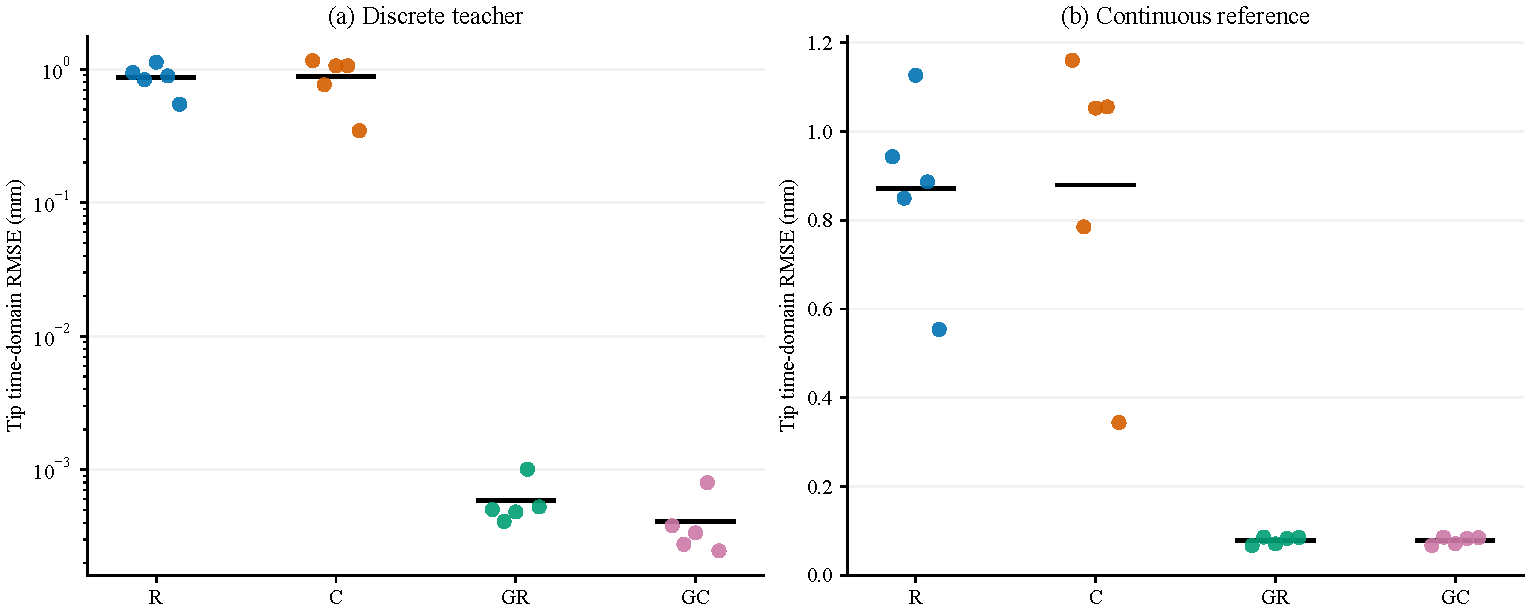
\includegraphics[width=0.96\textwidth]{neural_comparison.pdf}
\caption{端到端网络的杆端位移时间域RMSE。每个点表示一个独立数据与训练种子，黑线表示均值。左：相对式（36）离散教师；右：相对独立连续参考。四组均使用673个实参数和10000次更新；实复网络的具体函数类不同。}
\label{fig:neural}
\end{figure*}

\subsection{纯物理基线与端到端步长敏感性}
为进一步区分二次先验与学习残差的作用，将网络与零参数基线$H_0$比较：原步长$h$下，$H_0$对连续参考的杆端RMSE为$77.466\pm8.552\,\mu\mathrm m$，与GR（$78.263\pm8.899\,\mu\mathrm m$）和GC（$78.298\pm8.670\,\mu\mathrm m$）同处一水平。训练区内非线性与线性回复力$L^2$比仅$9.31\times10^{-6}$--$1.67\times10^{-5}$，与二次主部主导振动的设置一致。这些对照支持：在所测弱非线性区间和原步长下，已知二次物理信息解释了相对无先验网络的主要改善；学习残差的额外作用仍需结合步长、参照解和评价指标判断。

固定权重的步长加密（表\ref{tab:neural_refinement}、图\ref{fig:neural_physics_refinement}）进一步解耦残差与积分误差：$H_0$、GR与GC连续杆端误差随步长减小同步下降，至$h/4$时$H_0$在五种子中仍全部更优；到$h/8$，三者分别为$1.563\pm0.342$、$1.335\pm0.342$和$1.287\pm0.129\,\mu\mathrm m$，配对差$H_0-\mathrm{GR}$（$0.228\pm0.445\,\mu\mathrm m$）与$H_0-\mathrm{GC}$（$0.276\pm0.276\,\mu\mathrm m$）各在4/5种子为正。但完整状态相对$L^2$误差在$h/8$下仍由$H_0$（约$0.001353$）在全部五种子中低于GR（$0.002075$）与GC（$0.002104$），表明杆端投影微弱收益不代表全状态更优；无先验R、C在$h/8$下仍约$0.870$与$0.880\,\mathrm{mm}$（相对同步长教师，$H_0$、GR、GC恒定约$1.65$、$0.59$、$0.41\,\mu\mathrm m$，部分步长存在模型与积分误差抵消）。第\ref{sec:kam}节据此定量比对物理频移与离散频差。

\begin{table*}[t]
\centering
\caption{固定网络权重的步长加密结果。杆端误差单位为 $\mu\mathrm{m}$，报告五种子均值与样本标准差。}
\label{tab:neural_refinement}
\small
\begin{tabular}{llrrrr}
\toprule
比较对象 & 模型 & $h$ & $h/2$ & $h/4$ & $h/8$ \\
\midrule
连续参考 & $H_0$（无网络） & 77.466 $\pm$ 8.552 & 18.836 $\pm$ 2.048 & 4.350 $\pm$ 0.442 & 1.563 $\pm$ 0.342 \\
连续参考 & GR & 78.263 $\pm$ 8.899 & 19.596 $\pm$ 2.396 & 4.891 $\pm$ 0.777 & 1.335 $\pm$ 0.342 \\
连续参考 & GC & 78.298 $\pm$ 8.670 & 19.628 $\pm$ 2.157 & 4.908 $\pm$ 0.522 & 1.287 $\pm$ 0.129 \\
\midrule
同步长教师 & $H_0$（无网络） & 1.645 $\pm$ 0.471 & 1.647 $\pm$ 0.471 & 1.647 $\pm$ 0.471 & 1.647 $\pm$ 0.471 \\
同步长教师 & GR & 0.585 $\pm$ 0.239 & 0.586 $\pm$ 0.239 & 0.586 $\pm$ 0.240 & 0.586 $\pm$ 0.240 \\
同步长教师 & GC & 0.408 $\pm$ 0.225 & 0.408 $\pm$ 0.225 & 0.408 $\pm$ 0.226 & 0.408 $\pm$ 0.226 \\
\bottomrule
\end{tabular}
\par\smallskip\footnotesize 所有模型使用相同的八条测试轨迹、914个输出时刻和实际时长15.993 s；各轨迹先计算时间RMSE，再在种子内平均。$h=0.009999813692$ 为无量纲步长。同步长教师由完整非线性Hamiltonian在相同步长下求解；连续参考保持原DOP853解。最细步长的完整状态相对$L^2$误差为：$H_0$ $0.001353\pm0.000101$，GR $0.002075\pm0.000663$，GC $0.002104\pm0.000202$；该指标中$H_0$更低。R/C的完整结果随复现数据提供。
\end{table*}

\begin{figure*}[t]
\centering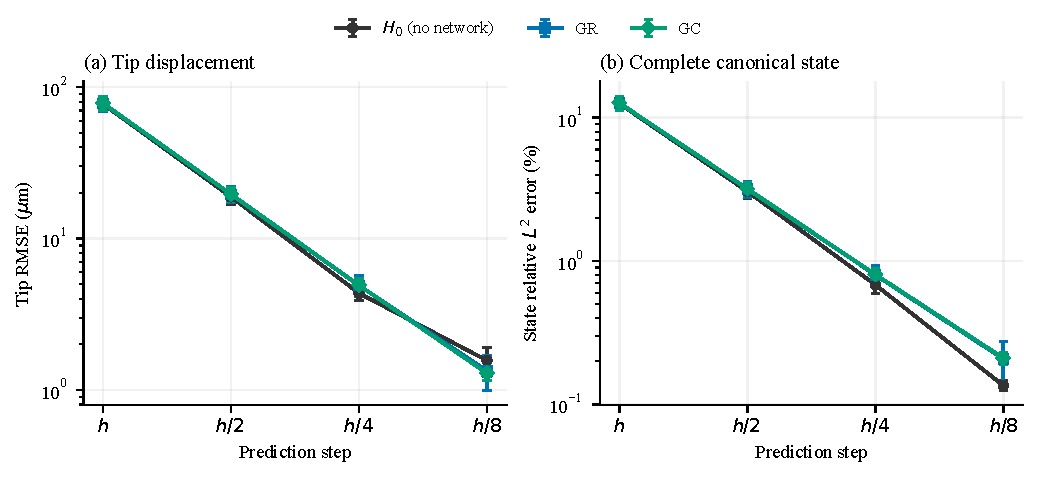
\includegraphics[width=0.95\textwidth]{neural_physics_refinement.pdf}
\caption{端到端模型与无网络物理基线的步长敏感性。全部五种子的权重、测试初值、输出时刻和15.993秒预测时域保持固定。左：对独立连续参考的杆端时间域RMSE；右：完整状态相对$L^2$误差。误差线为五种子的样本标准差。两种指标的排序不同；逐种子结果及R、C的全部步长数据随文提供。}
\label{fig:neural_physics_refinement}
\end{figure*}
